\documentclass{fkssolpub}

\usepackage[czech]{babel}
\usepackage{fontspec}
\usepackage{fkssugar}
\usepackage{amsmath}
\usepackage{graphicx}

\author{Ondřej Sedláček}
\school{Gymnázium Oty Pavla} 
\series{3p}
\problem{4} 

\begin{document} 

\begin{figure}[h!]
  \centering
  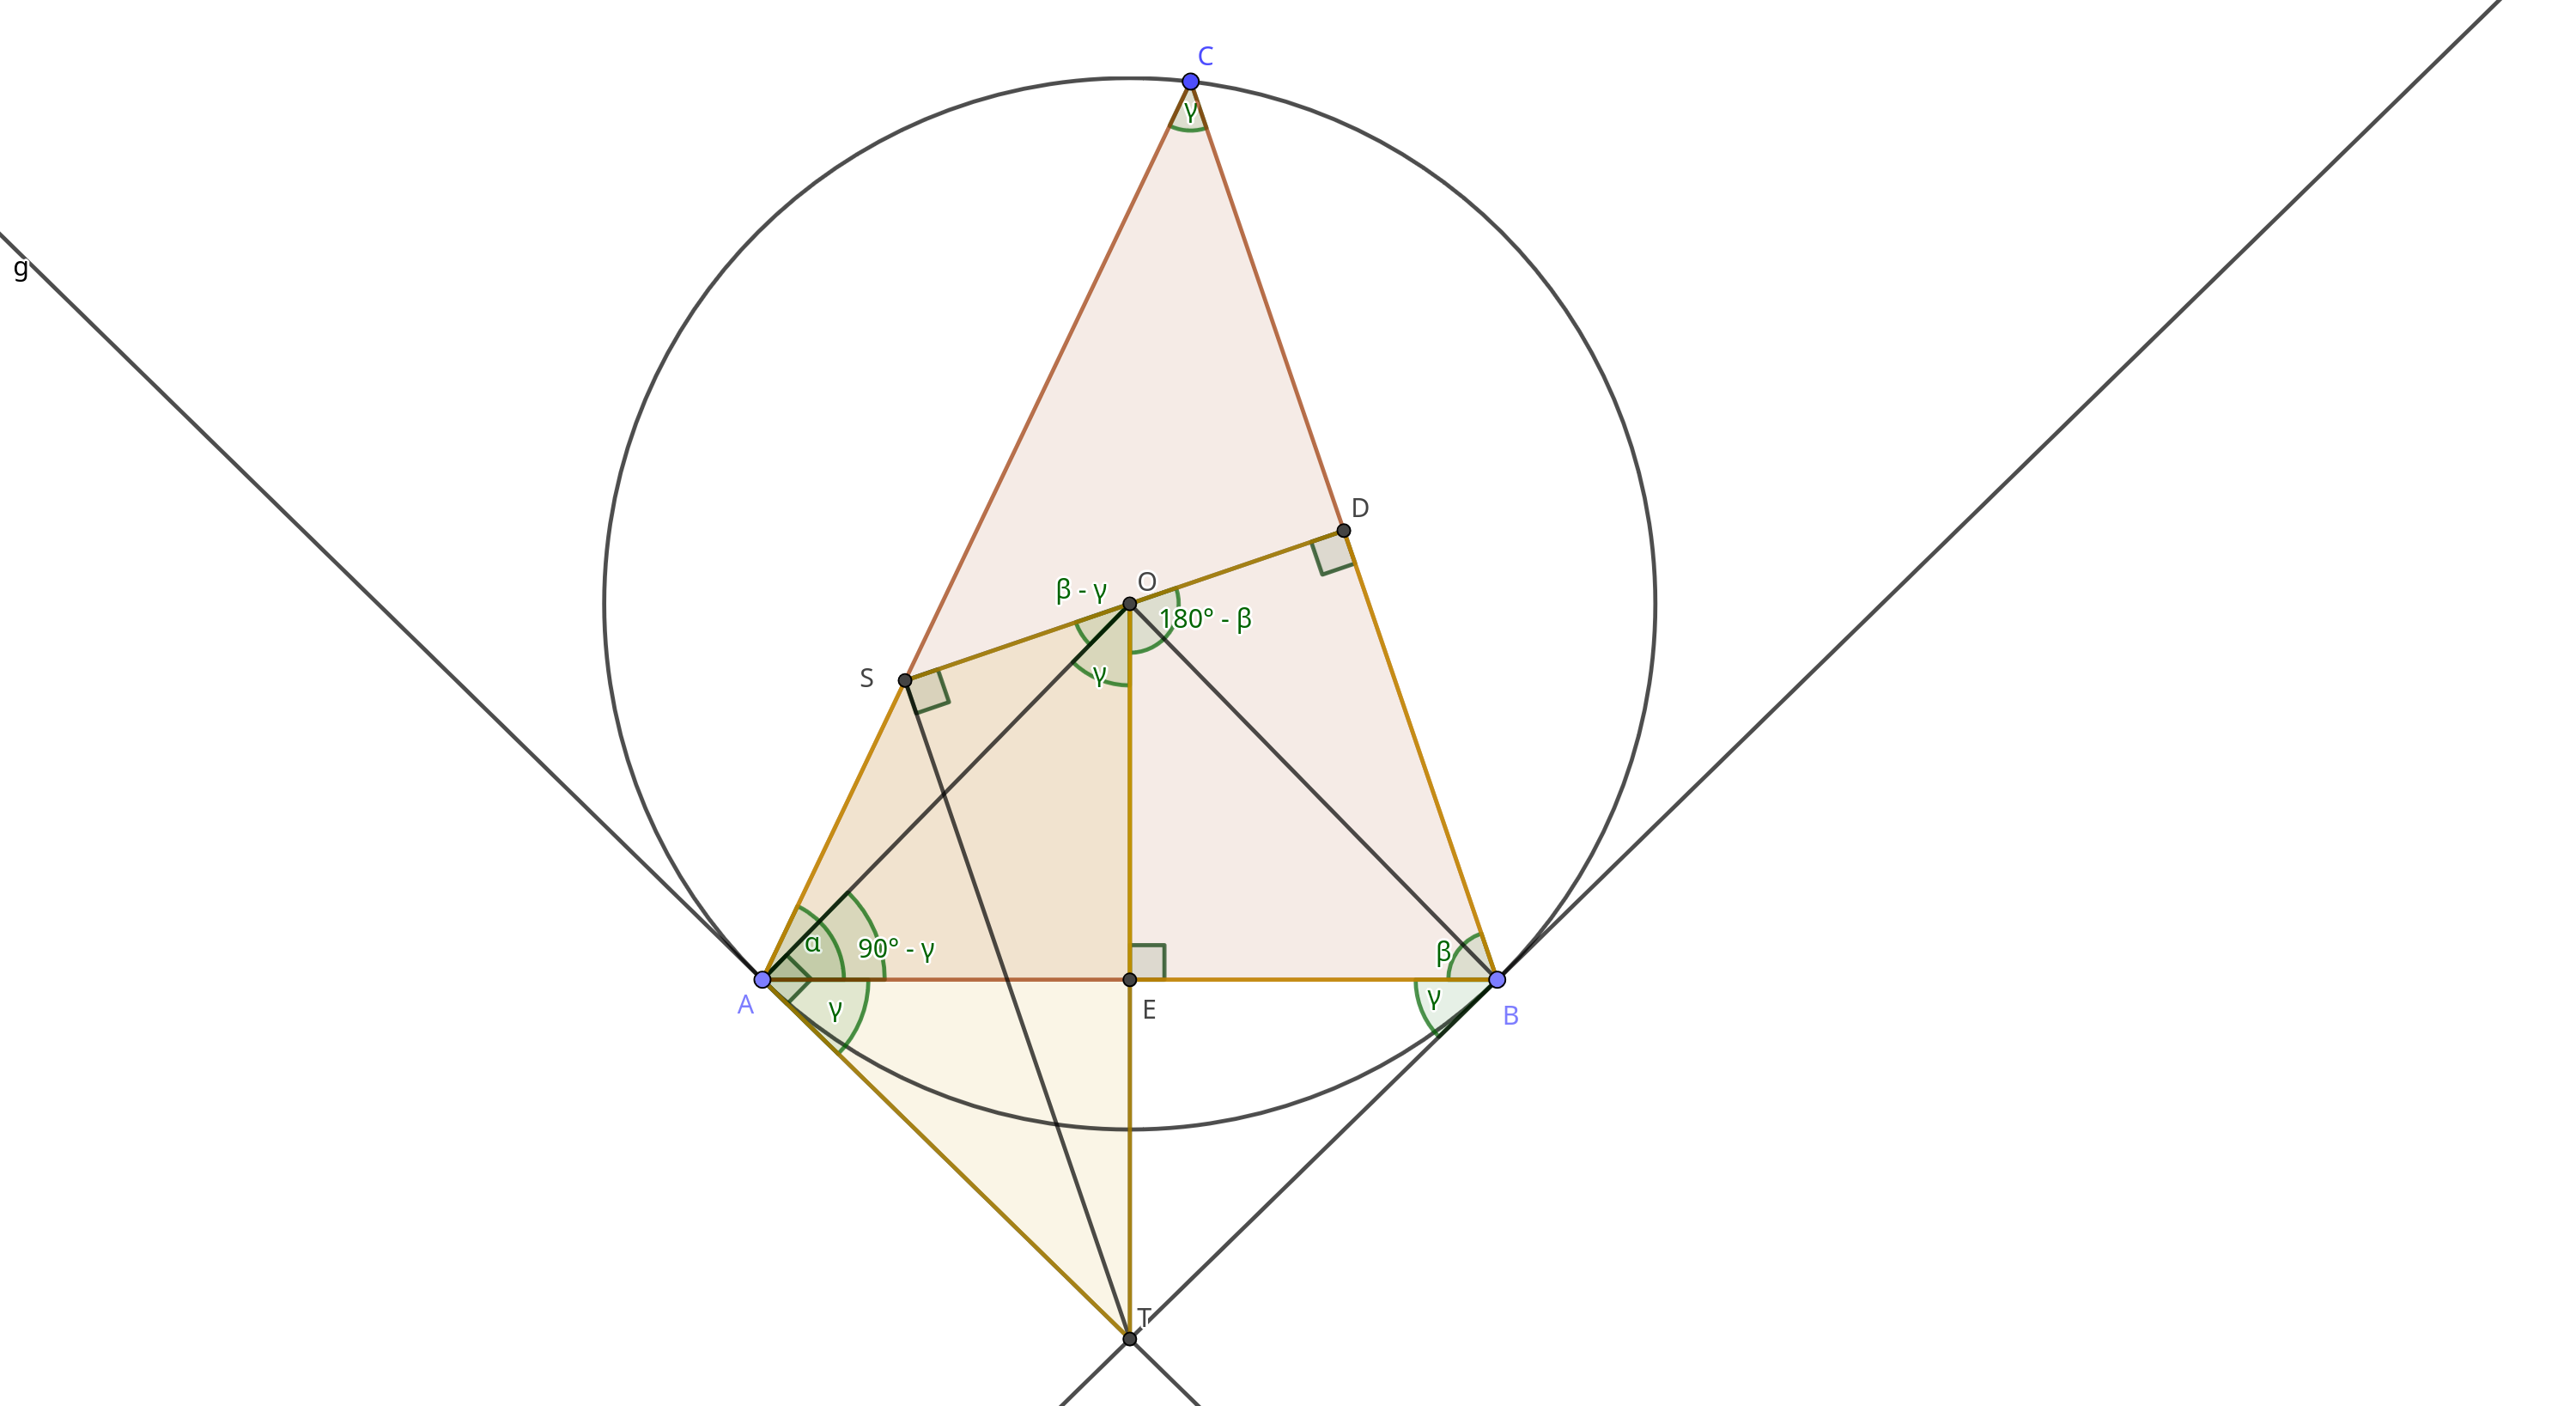
\includegraphics{4-fig.png}
  \caption{Konstrukce ze zadání s dopočítanými úhly}
\end{figure}

Protože víme, že osa strany BC je kolmá ke straně BC, potřebujeme dokázat, že
$ST \perp DS$, neboli $|\angle OST| = 90^{\circ}$.

Jako první dokážeme, že trojúhelník ABT je rovnoramenný se základnou AB. Díky větě
o úsekovém úhlu platí, že $|\angle ACB| = \gamma = |\angle TAB| = |\angle ABT|$,
tudíž je trojúhelník ABT nutně rovnoramenný. Díky tomu zřejmě osa strany AB
prochází bodem T, což využijeme dál při důkazu.

Následně můžeme dopočítat přes úhel $\angle BAO$, že úhel $|\angle AOT| = \gamma$,
protože $AT \perp AO$. Dále si však všimneme, že čtyřúhelník EBDO je tětivový,
protože $|\angle BEO| + |\angle ODB| = 180^{\circ}$, tím pádem je protější
úhel u středu opsané kružnice $|\angle DOE| = 180^{\circ} - \beta$.

Potom dopočítáme $|\angle AOS| = \beta - \gamma$. Díky tomu je čtyřúhelník
ATOS tětivový, protože $|\angle SAT| + |\angle TOS| = \alpha + \gamma + (\beta - \gamma)
+ \gamma = 180^{\circ}$. Díky tomu musí nutně platit $|\angle OAT| = |\angle OST|$.
A poněvadž $AT \perp AO$, je tedy $|\angle OST| = 90^{\circ}$.

Tím pádem je přímka ST rovnoběžná se stranou BC. Q. E. D.

\end{document}
